\section{Results and analysis}\label{sec:result}

We implemented our algorithm ($RTPD$) on three different RTX platforms: NVIDIA RTX 2080, NVIDIA RTX 3080, and NVIDIA RTX 4080, which are based on the Turing, Ampere, and Ada Lovelace architectures, respectively (Table~\ref{table:GPUs}).

\begin{table}[t]
\centering
\caption{Main specifications of GPUs used in experiments}
\label{table:GPUs}
\small
\begin{tabular}{|c|c|c|c|}
\hline
GPU                  & RTX2080 & RTX3080 & RTX4080      \\ \hline
Architecture         & Turing  & Ampere  & Ada Lovelace \\ \hline
\# of CUDA   cores   & 2,944    & 8,704    & 9,728        \\ \hline
CUDA core clock             & 1515 Mhz      & 1450 Mhz      & 2205 Mhz           \\ \hline
\# of RT cores        & 46      & 68      & 76           \\ \hline
RT core generation & 1st     & 2nd     & 3rd          \\ \hline
\end{tabular}%
\end{table}

%For comparison and to highlight the advantages of RT cores, we also tested on a non-RTX platform, the NVIDIA GTX 1080, which utilizes standard CUDA cores instead of RT cores for running RT-based algorithms.

%using three different NVIDIA RTX GPUs: NVIDIA RTX 2080, NVIDIA RTX 3080, and NVIDIA RTX 4080.
%Additionally, we report the performance on the NVIDIA GTX 1080 GPU, a non-RTX platform.
%All test environment consists the Intel i5-14600K 3.5GHz and 32GB memory.
%We employed CUDA 12.3, OptiX SDK 7.4.0, and NVIDIA thrust library to implement GPU algorithms.

To compare the performance of our method with previous work and conventional GPU implementations, we implemented two alternative methods:

%To verify the benefit of our methods, we implemented a $baseline$ algorithm, GPU-based naive approach, and RT-based methods.

\begin{itemize}
    %\item $CPU_{zheng}$ is an implementation based on Zheng et al.'s Hausdorff method, which operates on the CPU~\cite{zheng2022economic}.
    %However, instead of using the collision detection-based approach employed by Tang et al.~\cite{SIG09HIST}, we implemented a KD-tree-based PIP algorithm using the CGAL library, as it demonstrated better performance.
    %For penetration surface generation, we used a Map data structure for efficient processing on the CPU.
    \item $CPU_{Tang}$ is an implementation of Tang et al.'s method~\cite{SIG09HIST}, with performance further improved by applying Zheng et al.'s upper bound estimation method~\cite{zheng2022economic}.
    However, instead of using the collision detection and hole-filling approaches employed by Tang et al., we implemented a KD-tree-based PIP algorithm using the CGAL library and a Map data structure-based penetration surface generation algorithm, as these demonstrated better performance.
    
    \item $GPU_{cuda}$ is an implementation of the PD algorithm that runs on CUDA cores.
    We adapted an acceleration hierarchy, commonly used in proximity computation~\cite{lauterbach2010gproximity}, to both the PIP and PD stages.
    \revision{We utilized Quantized Bounding Volume Hierarchies (QBVH4) for their proven efficiency on GPUs~\cite{wald2019rtx}, building them directly on the GPU.
    Specifically, we sort the triangles using Morton codes when reading the object and then build the tree in a bottom-up manner.}
    For PD computation, we designed the system so that each thread handles a query point, maximizing the GPU’s parallel computing capabilities.
    For penetration surface generation, we employed our GPU-based algorithm presented in Sec.~\ref{subsec:surfaceGen}, enabling $GPU_{cuda}$ to execute entirely on the GPU.
    %To compute the Hausdorff distance, the previous research~\cite{zheng2022economic} is a sequential process, therefore we couldn`t implement the tree traverse in parallel, in other words, we implemented brute force approaches of the Hausdorff distance because of not suitable for GPU architecture.

%    \item $RTPD$ is an implementation of our algorithm with RT-core. We use the proposed \textit{AABB sampling} for the RT-based Hausdorff distance.
\end{itemize}

All test systems were equipped with identical CPUs (Intel i5-14600K) and 32GB of system memory.
For implementing our method and the alternatives, we used CUDA 12.3, Optix SDK 7.4, and the NVIDIA Thrust Library.

\textbf{Benchmarks: }
We established four distinct benchmark scenes using well-known models ranging in size from 50K to 12M triangles.
Each model was preprocessed using a hole-filling algorithm to ensure the objects were closed.
For each benchmark, we positioned two identical objects differently to achieve varying overlap ratios from 0.1 to 0.9.
Table~\ref{table_bench} provides detailed information about these benchmarks.
We established the ground truth for penetration depth through a brute-force computation of all vertex pairs, carefully separating overlapping volumes into distinct regions to account for the potential complexity of objects with multiple overlapping areas.

%%%
\begin{table*}[]
\centering
\caption{Benchmark scenes used in the experiments, showcasing various overlap ratios for different models.
The black lines represent the ground truth penetration depths, while the white lines indicate the results obtained using our method.}
\label{table_bench}
\small
%\resizebox{\textwidth}{!}{%
\begin{tabular}{@{}c|c|@{}m{2.7cm}@{ }m{2.7cm}@{ }m{2.7cm}@{ }m{2.7cm}@{ }m{2.7cm}@{ }m{2.7cm}@{ }m{2.7cm}@{ }m{2.7cm}@{}}
\hline
\multirow{2}{*}{Benchmark} & \# of Vtx. (\# of Tri.) & \multicolumn{5}{c}{Scene (overlap ratio)} \\  \cline{3-7}
    & per object              
    & \multicolumn{1}{c}{0.1}
    & \multicolumn{1}{c}{0.3}
    & \multicolumn{1}{c}{0.5}
    & \multicolumn{1}{c}{0.7}
    & \multicolumn{1}{c}{0.9}
    \\ \hline
{$Bunny$}                    & 0.26M (0.53M)           
    & \includegraphics[width=\linewidth]{Image/GT/bunny_10.png}   
    & \includegraphics[width=\linewidth]{Image/GT/bunny_30.png}       
    & \includegraphics[width=\linewidth]{Image/GT/bunny_50.png}        
    & \includegraphics[width=\linewidth]{Image/GT/bunny_70.png}        
    & \includegraphics[width=\linewidth]{Image/GT/bunny_90.png}       
    \\ \hline
{$David$}                     & 0.44M (0.88M)            
    & \includegraphics[width=\linewidth]{Image/GT/david_10.png}   
    & \includegraphics[width=\linewidth]{Image/GT/david_30.png}       
    & \includegraphics[width=\linewidth]{Image/GT/david_50.png}        
    & \includegraphics[width=\linewidth]{Image/GT/david_70.png}        
    & \includegraphics[width=\linewidth]{Image/GT/david_90.png}       
    \\ \hline
{$St.~Matthew$}                 & 5.96M (11.92M)          
    & \includegraphics[width=\linewidth]{Image/GT/stmatthew_10.png}   
    & \includegraphics[width=\linewidth]{Image/GT/stmatthew_30.png}       
    & \includegraphics[width=\linewidth]{Image/GT/stmatthew_50.png}        
    & \includegraphics[width=\linewidth]{Image/GT/stmatthew_70.png}        
    & \includegraphics[width=\linewidth]{Image/GT/stmatthew_90.png}       
    \\ \hline
{$Lucy$}                     & 6.42M (12.85M)          
    & \includegraphics[width=\linewidth]{Image/GT/lucy_10.png}   
    & \includegraphics[width=\linewidth]{Image/GT/lucy_30.png}       
    & \includegraphics[width=\linewidth]{Image/GT/lucy_50.png}        
    & \includegraphics[width=\linewidth]{Image/GT/lucy_70.png}        
    & \includegraphics[width=\linewidth]{Image/GT/lucy_90.png}       
    \\ \hline
\end{tabular}%
%}
\end{table*}

%%%

%It's important to note that the process of separating overlap volumes is highly time-intensive, often exceeding the time required for the penetration depth calculation itself.
%Previous studies typically presuppose or preprocess this aspect without accounting for the time involved.
%Conversely, in our experiments, we refrained from performing such preprocessing to ensure an accurate assessment of the actual performance and precision of our method and its alternatives.

%The PIP algorithms need a watertight mesh however some polygon has holes because they are built as 3D scans. Therefore, To avoid the failure of PIP, we did hole-filling algorithms and re-meshing on Blender.
%These results can be seen in Table~\ref{table:dataset} and Figure~\ref{fig:image_result}.
%To verify our methods, we set the benchmark scenarios as follows: Initially, we copied the polygon model, and then repositioned it by moving half the model's width to the side. Subsequently, we let it drop for 120 frames from a height equivalent to the model's height. This procedure ensured that the two models overlapped by approximately half the width.

\Skip{
\begin{figure*}[htb!]
    \centering
    \includegraphics[width=0.9\textwidth]{Image/result_image.pdf}
    \caption{Visualization of penetration depth result using $baseline$ and $RTPD$.}
    \label{fig:image_result}
\end{figure*}
}


\subsection{Results}

%%%
% Please add the following required packages to your document preamble:
% \usepackage{multirow}
% \usepackage{graphicx}
\begin{table*}[]
\centering
\small
\caption{This table shows the computation times (in milliseconds) for penetration depth using three different algorithms across four benchmarks.}
\label{table:result}
%\resizebox{\textwidth}{!}{%
\begin{tabular}{cccccccccccc}
\hline
\multicolumn{2}{|c|}{Benchmark} &
  \multicolumn{5}{c|}{$Bunny$} &
  \multicolumn{5}{c|}{$David$} \\ \hline
\multicolumn{2}{|c|}{Overlap ratio} &
  \multicolumn{1}{c|}{0.1} &
  \multicolumn{1}{c|}{0.3} &
  \multicolumn{1}{c|}{0.5} &
  \multicolumn{1}{c|}{0.7} &
  \multicolumn{1}{c|}{0.9} &
  \multicolumn{1}{c|}{0.1} &
  \multicolumn{1}{c|}{0.3} &
  \multicolumn{1}{c|}{0.5} &
  \multicolumn{1}{c|}{0.7} &
  \multicolumn{1}{c|}{0.9} \\ \hline
\multicolumn{2}{|c|}{$CPU_{Tang}$} &
  \multicolumn{1}{c|}{1,349.97} &
  \multicolumn{1}{c|}{1,971.65} &
  \multicolumn{1}{c|}{2,494.34} &
  \multicolumn{1}{c|}{2,923.93} &
  \multicolumn{1}{c|}{3,397.98} &
  \multicolumn{1}{c|}{2,530.55} &
  \multicolumn{1}{c|}{3,822.21} &
  \multicolumn{1}{c|}{5,280.25} &
  \multicolumn{1}{c|}{5,944.63} &
  \multicolumn{1}{c|}{6,525.23} \\ \hline
\multicolumn{1}{|c|}{\multirow{2}{*}{\begin{tabular}[c]{@{}c@{}}RTX\\ 2080\end{tabular}}} &
  \multicolumn{1}{c|}{$GPU_{cuda}$} &
  \multicolumn{1}{c|}{335.21} &
  \multicolumn{1}{c|}{540.96} &
  \multicolumn{1}{c|}{611.64} &
  \multicolumn{1}{c|}{760.13} &
  \multicolumn{1}{c|}{854.56} &
  \multicolumn{1}{c|}{487.52} &
  \multicolumn{1}{c|}{877.72} &
  \multicolumn{1}{c|}{1,382.58} &
  \multicolumn{1}{c|}{1,515.79} &
  \multicolumn{1}{c|}{1,780.15} \\ \cmidrule{2-12} 
\multicolumn{1}{|c|}{} &
  \multicolumn{1}{c|}{$RTPD$} &
  \multicolumn{1}{c|}{81.73} &
  \multicolumn{1}{c|}{138.68} &
  \multicolumn{1}{c|}{179.45} &
  \multicolumn{1}{c|}{204.48} &
  \multicolumn{1}{c|}{247.02} &
  \multicolumn{1}{c|}{140.53} &
  \multicolumn{1}{c|}{243.06} &
  \multicolumn{1}{c|}{394.40} &
  \multicolumn{1}{c|}{457.15} &
  \multicolumn{1}{c|}{529.75} \\ \hline
\multicolumn{1}{|c|}{\multirow{2}{*}{\begin{tabular}[c]{@{}c@{}}RTX\\ 3080\end{tabular}}} &
  \multicolumn{1}{c|}{$GPU_{cuda}$} &
  \multicolumn{1}{c|}{170.72} &
  \multicolumn{1}{c|}{279.66} &
  \multicolumn{1}{c|}{305.27} &
  \multicolumn{1}{c|}{376.56} &
  \multicolumn{1}{c|}{432.13} &
  \multicolumn{1}{c|}{272.39} &
  \multicolumn{1}{c|}{384.01} &
  \multicolumn{1}{c|}{658.94} &
  \multicolumn{1}{c|}{711.40} &
  \multicolumn{1}{c|}{833.11} \\ \cmidrule{2-12} 
\multicolumn{1}{|c|}{} &
  \multicolumn{1}{c|}{$RTPD$} &
  \multicolumn{1}{c|}{87.55} &
  \multicolumn{1}{c|}{128.08} &
  \multicolumn{1}{c|}{165.00} &
  \multicolumn{1}{c|}{177.69} &
  \multicolumn{1}{c|}{213.25} &
  \multicolumn{1}{c|}{130.08} &
  \multicolumn{1}{c|}{208.98} &
  \multicolumn{1}{c|}{310.78} &
  \multicolumn{1}{c|}{375.77} &
  \multicolumn{1}{c|}{420.57} \\ \hline
\multicolumn{1}{|c|}{\multirow{2}{*}{\begin{tabular}[c]{@{}c@{}}RTX\\ 4080\end{tabular}}} &
  \multicolumn{1}{c|}{$GPU_{cuda}$} &
  \multicolumn{1}{c|}{113.49} &
  \multicolumn{1}{c|}{148.10} &
  \multicolumn{1}{c|}{157.05} &
  \multicolumn{1}{c|}{175.48} &
  \multicolumn{1}{c|}{191.35} &
  \multicolumn{1}{c|}{133.69} &
  \multicolumn{1}{c|}{200.61} &
  \multicolumn{1}{c|}{291.89} &
  \multicolumn{1}{c|}{309.29} &
  \multicolumn{1}{c|}{347.82} \\ \cmidrule{2-12} 
\multicolumn{1}{|c|}{} &
  \multicolumn{1}{c|}{$RTPD$} &
  \multicolumn{1}{c|}{69.60} &
  \multicolumn{1}{c|}{95.83} &
  \multicolumn{1}{c|}{121.98} &
  \multicolumn{1}{c|}{138.94} &
  \multicolumn{1}{c|}{163.73} &
  \multicolumn{1}{c|}{108.91} &
  \multicolumn{1}{c|}{172.60} &
  \multicolumn{1}{c|}{246.23} &
  \multicolumn{1}{c|}{288.23} &
  \multicolumn{1}{c|}{323.81} \\ \hline
\multicolumn{1}{l}{} &
  \multicolumn{1}{l}{} &
  \multicolumn{1}{l}{} &
  \multicolumn{1}{l}{} &
  \multicolumn{1}{l}{} &
  \multicolumn{1}{l}{} &
  \multicolumn{1}{l}{} &
  \multicolumn{1}{l}{} &
  \multicolumn{1}{l}{} &
  \multicolumn{1}{l}{} &
  \multicolumn{1}{l}{} &
  \multicolumn{1}{l}{} \\ \hline
\multicolumn{2}{|c|}{Benchmark} &
  \multicolumn{5}{c|}{$stmatthew$} &
  \multicolumn{5}{c|}{$Lucy$} \\ \hline
\multicolumn{2}{|c|}{Overlap ratio} &
  \multicolumn{1}{c|}{0.1} &
  \multicolumn{1}{c|}{0.3} &
  \multicolumn{1}{c|}{0.5} &
  \multicolumn{1}{c|}{0.7} &
  \multicolumn{1}{c|}{0.9} &
  \multicolumn{1}{c|}{0.1} &
  \multicolumn{1}{c|}{0.3} &
  \multicolumn{1}{c|}{0.5} &
  \multicolumn{1}{c|}{0.7} &
  \multicolumn{1}{c|}{0.9} \\ \hline
\multicolumn{2}{|c|}{$CPU_{Tang}$} &
  \multicolumn{1}{c|}{20,814.80} &
  \multicolumn{1}{c|}{36,688.20} &
  \multicolumn{1}{c|}{46,477.20} &
  \multicolumn{1}{c|}{57,628.90} &
  \multicolumn{1}{c|}{64,832.50} &
  \multicolumn{1}{c|}{72,682.00} &
  \multicolumn{1}{c|}{79,554.70} &
  \multicolumn{1}{c|}{102,890.00} &
  \multicolumn{1}{c|}{130,233.00} &
  \multicolumn{1}{c|}{147,261.00} \\ \hline
\multicolumn{1}{|c|}{\multirow{2}{*}{\begin{tabular}[c]{@{}c@{}}RTX\\ 2080\end{tabular}}} &
  \multicolumn{1}{c|}{$GPU_{cuda}$} &
  \multicolumn{1}{c|}{19,816.20} &
  \multicolumn{1}{c|}{36,432.50} &
  \multicolumn{1}{c|}{57,616.00} &
  \multicolumn{1}{c|}{73,974.10} &
  \multicolumn{1}{c|}{67,363.10} &
  \multicolumn{1}{c|}{16,738.50} &
  \multicolumn{1}{c|}{25,704.30} &
  \multicolumn{1}{c|}{40,311.40} &
  \multicolumn{1}{c|}{65,276.80} &
  \multicolumn{1}{c|}{73,633.70} \\ \cmidrule{2-12} 
\multicolumn{1}{|c|}{} &
  \multicolumn{1}{c|}{$RTPD$} &
  \multicolumn{1}{c|}{4,429.51} &
  \multicolumn{1}{c|}{9,193.99} &
  \multicolumn{1}{c|}{13,054.40} &
  \multicolumn{1}{c|}{18,727.20} &
  \multicolumn{1}{c|}{25,086.60} &
  \multicolumn{1}{c|}{3,138.68} &
  \multicolumn{1}{c|}{7,055.98} &
  \multicolumn{1}{c|}{13,021.90} &
  \multicolumn{1}{c|}{19,532.80} &
  \multicolumn{1}{c|}{24,348.70} \\ \hline
\multicolumn{1}{|c|}{\multirow{2}{*}{\begin{tabular}[c]{@{}c@{}}RTX\\ 3080\end{tabular}}} &
  \multicolumn{1}{c|}{$GPU_{cuda}$} &
  \multicolumn{1}{c|}{9,602.12} &
  \multicolumn{1}{c|}{18,445.30} &
  \multicolumn{1}{c|}{29,214.30} &
  \multicolumn{1}{c|}{38,252.20} &
  \multicolumn{1}{c|}{34,912.90} &
  \multicolumn{1}{c|}{8,002.66} &
  \multicolumn{1}{c|}{12,110.20} &
  \multicolumn{1}{c|}{19,306.90} &
  \multicolumn{1}{c|}{32,417.80} &
  \multicolumn{1}{c|}{36,425.80} \\ \cmidrule{2-12} 
\multicolumn{1}{|c|}{} &
  \multicolumn{1}{c|}{$RTPD$} &
  \multicolumn{1}{c|}{3,372.21} &
  \multicolumn{1}{c|}{6,538.83} &
  \multicolumn{1}{c|}{8,699.78} &
  \multicolumn{1}{c|}{11,846.90} &
  \multicolumn{1}{c|}{15,362.40} &
  \multicolumn{1}{c|}{2,401.75} &
  \multicolumn{1}{c|}{5,175.98} &
  \multicolumn{1}{c|}{8,911.14} &
  \multicolumn{1}{c|}{12,655.40} &
  \multicolumn{1}{c|}{14,554.30} \\ \hline
\multicolumn{1}{|c|}{\multirow{2}{*}{\begin{tabular}[c]{@{}c@{}}RTX\\ 4080\end{tabular}}} &
  \multicolumn{1}{c|}{$GPU_{cuda}$} &
  \multicolumn{1}{c|}{3,485.11} &
  \multicolumn{1}{c|}{5,928.27} &
  \multicolumn{1}{c|}{8,771.09} &
  \multicolumn{1}{c|}{10,682.00} &
  \multicolumn{1}{c|}{10,088.30} &
  \multicolumn{1}{c|}{3,055.14} &
  \multicolumn{1}{c|}{4,389.57} &
  \multicolumn{1}{c|}{6,637.78} &
  \multicolumn{1}{c|}{9,800.50} &
  \multicolumn{1}{c|}{10,311.70} \\ \cmidrule{2-12} 
\multicolumn{1}{|c|}{} &
  \multicolumn{1}{c|}{$RTPD$} &
  \multicolumn{1}{c|}{2,497.75} &
  \multicolumn{1}{c|}{4,786.06} &
  \multicolumn{1}{c|}{6,276.15} &
  \multicolumn{1}{c|}{8,434.39} &
  \multicolumn{1}{c|}{10,804.20} &
  \multicolumn{1}{c|}{1,930.04} &
  \multicolumn{1}{c|}{3,965.84} &
  \multicolumn{1}{c|}{6,678.99} &
  \multicolumn{1}{c|}{9,183.59} &
  \multicolumn{1}{c|}{10,637.80} \\ \hline
\end{tabular}%
%}
\end{table*}


\Skip{%%%%%%%%%%%%%%%%%%%%%%%%%%%%%%%%%%%%%%%%%%%
\begin{table*}[]
\centering
\caption{This table shows the computation times (in milliseconds) for penetration depth using three different algorithms across five scenes, each with varying overlap ratios.
The number in parentheses is the error rate over the ground truth.
"$Avg.$" denotes the average processing time computed across these five distinct scenes.}
\label{table:result}
\small
\resizebox{\textwidth}{!}{%
\begin{tabular}{cccccccccccccl}
\hline
\multicolumn{2}{|c||}{} &
  \multicolumn{6}{c||}{$Bunny$} &
  \multicolumn{6}{c|}{$David$} \\ \hline
\multicolumn{2}{|c||}{Overlap ratio} &
  \multicolumn{1}{c|}{0.1} &
  \multicolumn{1}{c|}{0.3} &
  \multicolumn{1}{c|}{0.5} &
  \multicolumn{1}{c|}{0.7} &
  \multicolumn{1}{c||}{0.9} &
  \multicolumn{1}{c||}{$Avg.$} &
  \multicolumn{1}{c|}{0.1} &
  \multicolumn{1}{c|}{0.3} &
  \multicolumn{1}{c|}{0.5} &
  \multicolumn{1}{c|}{0.7} &
  \multicolumn{1}{c||}{0.9} &
  \multicolumn{1}{c|}{$Avg.$} \\ \hline
\multicolumn{2}{|c||}{$CPU_{zheng}$} &
  \multicolumn{1}{c|}{1349.97} &
  \multicolumn{1}{c|}{1971.65} &
  \multicolumn{1}{c|}{2494.34} &
  \multicolumn{1}{c|}{2923.93} &
  \multicolumn{1}{c|}{3397.98} &
  \multicolumn{1}{c||}{2427.57} &
  \multicolumn{1}{c|}{2530.55} &
  \multicolumn{1}{c|}{3822.21} &
  \multicolumn{1}{c|}{5280.25} &
  \multicolumn{1}{c|}{5944.63} &
  \multicolumn{1}{c|}{6525.23} &
  \multicolumn{1}{c|}{4820.57} \\ \hline
\multicolumn{1}{|c|}{\multirow{2}{*}{\begin{tabular}[c]{@{}c@{}}GTX\\ 1080\end{tabular}}} &
  \multicolumn{1}{c||}{$GPU_{cuda}$} &
  \multicolumn{1}{c|}{865.12} &
  \multicolumn{1}{c|}{1697.44} &
  \multicolumn{1}{c|}{1957.23} &
  \multicolumn{1}{c|}{2516.23} &
  \multicolumn{1}{c|}{2924.40} &
  \multicolumn{1}{c||}{1992.08} &
  \multicolumn{1}{c|}{1413.49} &
  \multicolumn{1}{c|}{2966.87} &
  \multicolumn{1}{c|}{4948.63} &
  \multicolumn{1}{c|}{5510.86} &
  \multicolumn{1}{c|}{6426.93} &
  \multicolumn{1}{c|}{4253.36} \\ \cmidrule{2-14} 
\multicolumn{1}{|c|}{} &
  \multicolumn{1}{c||}{$RTPD$} &
  \multicolumn{1}{c|}{184.38} &
  \multicolumn{1}{c|}{203.57} &
  \multicolumn{1}{c|}{257.78} &
  \multicolumn{1}{c|}{290.78} &
  \multicolumn{1}{c|}{334.84} &
  \multicolumn{1}{c||}{254.27} &
  \multicolumn{1}{c|}{310.71} &
  \multicolumn{1}{c|}{396.89} &
  \multicolumn{1}{c|}{549.53} &
  \multicolumn{1}{c|}{634.38} &
  \multicolumn{1}{c|}{712.57} &
  \multicolumn{1}{c|}{520.82} \\ \hline
\multicolumn{1}{|c|}{\multirow{2}{*}{\begin{tabular}[c]{@{}c@{}}RTX\\ 2080\end{tabular}}} &
  \multicolumn{1}{c||}{$GPU_{cuda}$} &
  \multicolumn{1}{c|}{335.21} &
  \multicolumn{1}{c|}{540.96} &
  \multicolumn{1}{c|}{611.64} &
  \multicolumn{1}{c|}{760.13} &
  \multicolumn{1}{c|}{854.56} &
  \multicolumn{1}{c||}{620.50} &
  \multicolumn{1}{c|}{487.52} &
  \multicolumn{1}{c|}{877.72} &
  \multicolumn{1}{c|}{1382.58} &
  \multicolumn{1}{c|}{1515.79} &
  \multicolumn{1}{c|}{1780.15} &
  \multicolumn{1}{c|}{1208.75} \\ \cmidrule{2-14} 
\multicolumn{1}{|c|}{} &
  \multicolumn{1}{c||}{$RTPD$} &
  \multicolumn{1}{c|}{68.36} &
  \multicolumn{1}{c|}{95.98} &
  \multicolumn{1}{c|}{141.15} &
  \multicolumn{1}{c|}{131.02} &
  \multicolumn{1}{c|}{152.44} &
  \multicolumn{1}{c||}{111.79} &
  \multicolumn{1}{c|}{113.07} &
  \multicolumn{1}{c|}{182.26} &
  \multicolumn{1}{c|}{248.79} &
  \multicolumn{1}{c|}{290.93} &
  \multicolumn{1}{c|}{330.16} &
  \multicolumn{1}{c|}{233.04} \\ \hline
\multicolumn{1}{|c|}{\multirow{2}{*}{\begin{tabular}[c]{@{}c@{}}RTX\\ 3080\end{tabular}}} &
  \multicolumn{1}{c||}{$GPU_{cuda}$} &
  \multicolumn{1}{c|}{170.12} &
  \multicolumn{1}{c|}{279.66} &
  \multicolumn{1}{c|}{305.27} &
  \multicolumn{1}{c|}{376.56} &
  \multicolumn{1}{c|}{432.13} &
  \multicolumn{1}{c||}{312.87} &
  \multicolumn{1}{c|}{272.39} &
  \multicolumn{1}{c|}{384.01} &
  \multicolumn{1}{c|}{658.94} &
  \multicolumn{1}{c|}{711.40} &
  \multicolumn{1}{c|}{833.11} &
  \multicolumn{1}{c|}{571.97} \\ \cmidrule{2-14} 
\multicolumn{1}{|c|}{} &
  \multicolumn{1}{c||}{$RTPD$} &
  \multicolumn{1}{c|}{76.26} &
  \multicolumn{1}{c|}{93.23} &
  \multicolumn{1}{c|}{115.02} &
  \multicolumn{1}{c|}{124.70} &
  \multicolumn{1}{c|}{137.73} &
  \multicolumn{1}{c||}{109.39} &
  \multicolumn{1}{c|}{109.87} &
  \multicolumn{1}{c|}{156.62} &
  \multicolumn{1}{c|}{211.72} &
  \multicolumn{1}{c|}{240.52} &
  \multicolumn{1}{c|}{271.39} &
  \multicolumn{1}{c|}{198.02} \\ \hline
\multicolumn{1}{|c|}{\multirow{2}{*}{\begin{tabular}[c]{@{}c@{}}RTX\\ 4080\end{tabular}}} &
  \multicolumn{1}{c||}{$GPU_{cuda}$} &
  \multicolumn{1}{c|}{113.49} &
  \multicolumn{1}{c|}{148.10} &
  \multicolumn{1}{c|}{157.05} &
  \multicolumn{1}{c|}{175.48} &
  \multicolumn{1}{c|}{191.35} &
  \multicolumn{1}{c||}{157.10} &
  \multicolumn{1}{c|}{133.69} &
  \multicolumn{1}{c|}{200.61} &
  \multicolumn{1}{c|}{291.89} &
  \multicolumn{1}{c|}{309.29} &
  \multicolumn{1}{c|}{347.82} &
  \multicolumn{1}{c|}{256.66} \\ \cmidrule{2-14} 
\multicolumn{1}{|c|}{} &
  \multicolumn{1}{c||}{$RTPD$} &
  \multicolumn{1}{m{0.8cm}|}{65.49 (0.37\%)} &
  \multicolumn{1}{m{0.8cm}|}{77.93 (0.51\%)} &
  \multicolumn{1}{m{0.8cm}|}{93.45 (2.33\%)} &
  \multicolumn{1}{m{0.8cm}|}{102.91 (1.13\%)} &
  \multicolumn{1}{m{0.8cm}|}{125.15 (2.13\%)} &
  \multicolumn{1}{m{0.8cm}||}{92.99 (1.30\%)} &
  \multicolumn{1}{m{0.8cm}|}{107.24 (0.24\%)} &
  \multicolumn{1}{m{0.8cm}|}{130.24 (2.53\%)} &
  \multicolumn{1}{m{0.8cm}|}{179.83 (2.24\%)} &
  \multicolumn{1}{m{0.8cm}|}{200.28 (2.05\%)} &
  \multicolumn{1}{m{0.8cm}|}{217.31 (2.49\%)} &
  \multicolumn{1}{m{0.8cm}|}{166.98 (1.91\%)} \\ \hline
\multicolumn{1}{l}{} &
  \multicolumn{1}{l}{} &
  \multicolumn{1}{l}{} &
  \multicolumn{1}{l}{} &
  \multicolumn{1}{l}{} &
  \multicolumn{1}{l}{} &
  \multicolumn{1}{l}{} &
  \multicolumn{1}{l}{} &
  \multicolumn{1}{l}{} &
  \multicolumn{1}{l}{} &
  \multicolumn{1}{l}{} &
  \multicolumn{1}{l}{} &
  \multicolumn{1}{l}{} &
   \\ \hline
\multicolumn{2}{|c||}{} &
  \multicolumn{6}{c||}{$stmatthew$} &
  \multicolumn{6}{c|}{$Lucy$} \\ \hline
\multicolumn{2}{|c||}{Overlap ratio} &
  \multicolumn{1}{c|}{0.1} &
  \multicolumn{1}{c|}{0.3} &
  \multicolumn{1}{c|}{0.5} &
  \multicolumn{1}{c|}{0.7} &
  \multicolumn{1}{c||}{0.9} &
  \multicolumn{1}{c||}{$Avg.$} &
  \multicolumn{1}{c|}{0.1} &
  \multicolumn{1}{c|}{0.3} &
  \multicolumn{1}{c|}{0.5} &
  \multicolumn{1}{c|}{0.7} &
  \multicolumn{1}{c||}{0.9} &
  \multicolumn{1}{c|}{$Avg.$} \\ \hline
\multicolumn{2}{|c||}{$CPU_{zheng}$} &
  \multicolumn{1}{c|}{20814.80} &
  \multicolumn{1}{c|}{36688.20} &
  \multicolumn{1}{c|}{46477.20} &
  \multicolumn{1}{c|}{57628.90} &
  \multicolumn{1}{c|}{64832.50} &
  \multicolumn{1}{c||}{45288.32} &
  \multicolumn{1}{c|}{50257.40} &
  \multicolumn{1}{c|}{68900.90} &
  \multicolumn{1}{c|}{88975.10} &
  \multicolumn{1}{c|}{114271.00} &
  \multicolumn{1}{c|}{128525.90} &
  \multicolumn{1}{c|}{90185.88} \\ \hline
\multicolumn{1}{|c|}{\multirow{2}{*}{\begin{tabular}[c]{@{}c@{}}GTX\\ 1080\end{tabular}}} &
  \multicolumn{1}{c||}{$GPU_{cuda}$} &
  \multicolumn{1}{c|}{68807.10} &
  \multicolumn{1}{c|}{125239.00} &
  \multicolumn{1}{c|}{195639.00} &
  \multicolumn{1}{c|}{249668.00} &
  \multicolumn{1}{c|}{228803.00} &
  \multicolumn{1}{c||}{173631.22} &
  \multicolumn{1}{c|}{59005.10} &
  \multicolumn{1}{c|}{89240.20} &
  \multicolumn{1}{c|}{138818.00} &
  \multicolumn{1}{c|}{220256.00} &
  \multicolumn{1}{c|}{246241.00} &
  \multicolumn{1}{c|}{150712.06} \\ \cmidrule{2-14} 
\multicolumn{1}{|c|}{} &
  \multicolumn{1}{c||}{$RTPD$} &
  \multicolumn{1}{c|}{12494.40} &
  \multicolumn{1}{c|}{25981.50} &
  \multicolumn{1}{c|}{35302.40} &
  \multicolumn{1}{c|}{49190.50} &
  \multicolumn{1}{c|}{64053.30} &
  \multicolumn{1}{c||}{37404.42} &
  \multicolumn{1}{c|}{5227.55} &
  \multicolumn{1}{c|}{10360.60} &
  \multicolumn{1}{c|}{19236.60} &
  \multicolumn{1}{c|}{28242.70} &
  \multicolumn{1}{c|}{34888.10} &
  \multicolumn{1}{c|}{19591.11} \\ \hline
\multicolumn{1}{|c|}{\multirow{2}{*}{\begin{tabular}[c]{@{}c@{}}RTX\\ 2080\end{tabular}}} &
  \multicolumn{1}{c||}{$GPU_{cuda}$} &
  \multicolumn{1}{c|}{19816.20} &
  \multicolumn{1}{c|}{36432.50} &
  \multicolumn{1}{c|}{57616.00} &
  \multicolumn{1}{c|}{73974.10} &
  \multicolumn{1}{c|}{67363.10} &
  \multicolumn{1}{c||}{51040.38} &
  \multicolumn{1}{c|}{16738.50} &
  \multicolumn{1}{c|}{25704.30} &
  \multicolumn{1}{c|}{40311.40} &
  \multicolumn{1}{c|}{65276.80} &
  \multicolumn{1}{c|}{73633.70} &
  \multicolumn{1}{c|}{44332.94} \\ \cmidrule{2-14} 
\multicolumn{1}{|c|}{} &
  \multicolumn{1}{c||}{$RTPD$} &
  \multicolumn{1}{c|}{4527.32} &
  \multicolumn{1}{c|}{9379.19} &
  \multicolumn{1}{c|}{13443.60} &
  \multicolumn{1}{c|}{19310.20} &
  \multicolumn{1}{c|}{25588.70} &
  \multicolumn{1}{c||}{14449.80} &
  \multicolumn{1}{c|}{2137.31} &
  \multicolumn{1}{c|}{4455.35} &
  \multicolumn{1}{c|}{7712.70} &
  \multicolumn{1}{c|}{10925.70} &
  \multicolumn{1}{c|}{13186.80} &
  \multicolumn{1}{c|}{7683.57} \\ \hline
\multicolumn{1}{|c|}{\multirow{2}{*}{\begin{tabular}[c]{@{}c@{}}RTX\\ 3080\end{tabular}}} &
  \multicolumn{1}{c||}{$GPU_{cuda}$} &
  \multicolumn{1}{c|}{9602.12} &
  \multicolumn{1}{c|}{18445.30} &
  \multicolumn{1}{c|}{29214.30} &
  \multicolumn{1}{c|}{38252.20} &
  \multicolumn{1}{c|}{34912.90} &
  \multicolumn{1}{c||}{26085.36} &
  \multicolumn{1}{c|}{8002.66} &
  \multicolumn{1}{c|}{12110.20} &
  \multicolumn{1}{c|}{19306.90} &
  \multicolumn{1}{c|}{32417.80} &
  \multicolumn{1}{c|}{36425.80} &
  \multicolumn{1}{c|}{21652.67} \\ \cmidrule{2-14} 
\multicolumn{1}{|c|}{} &
  \multicolumn{1}{c||}{$RTPD$} &
  \multicolumn{1}{c|}{3281.90} &
  \multicolumn{1}{c|}{6458.25} &
  \multicolumn{1}{c|}{8650.91} &
  \multicolumn{1}{c|}{11885.10} &
  \multicolumn{1}{c|}{15252.90} &
  \multicolumn{1}{c||}{9105.81} &
  \multicolumn{1}{c|}{1606.30} &
  \multicolumn{1}{c|}{3286.01} &
  \multicolumn{1}{c|}{5549.25} &
  \multicolumn{1}{c|}{7646.50} &
  \multicolumn{1}{c|}{8920.07} &
  \multicolumn{1}{c|}{5401.63} \\ \hline
\multicolumn{1}{|c|}{\multirow{2}{*}{\begin{tabular}[c]{@{}c@{}}RTX\\ 4080\end{tabular}}} &
  \multicolumn{1}{c||}{$GPU_{cuda}$} &
  \multicolumn{1}{c|}{3485.11} &
  \multicolumn{1}{c|}{5928.27} &
  \multicolumn{1}{c|}{8771.09} &
  \multicolumn{1}{c|}{10682.00} &
  \multicolumn{1}{c|}{10088.30} &
  \multicolumn{1}{c||}{7790.95} &
  \multicolumn{1}{c|}{3055.14} &
  \multicolumn{1}{c|}{4389.57} &
  \multicolumn{1}{c|}{6637.78} &
  \multicolumn{1}{c|}{9800.50} &
  \multicolumn{1}{c|}{10311.70} &
  \multicolumn{1}{c|}{6838.94} \\ \cmidrule{2-14} 
\multicolumn{1}{|c|}{} &
  \multicolumn{1}{c||}{$RTPD$} &
  \multicolumn{1}{c|}{2581.62} &
  \multicolumn{1}{c|}{4911.31} &
  \multicolumn{1}{c|}{6444.12} &
  \multicolumn{1}{c|}{8657.64} &
  \multicolumn{1}{c|}{10987.70} &
  \multicolumn{1}{c||}{6716.48} &
  \multicolumn{1}{c|}{1334.76} &
  \multicolumn{1}{c|}{2588.09} &
  \multicolumn{1}{c|}{4252.41} &
  \multicolumn{1}{c|}{5784.73} &
  \multicolumn{1}{c|}{6714.60} &
  \multicolumn{1}{c|}{4134.92} \\ \hline
\end{tabular}%
}
\end{table*}
}
%%%%%%%%%%%%%%%%%%%%%%%%%%%%%%%%%%%%%%%%%%%%%%%%%%
%%%

Table~\ref{table:result} displays the processing times for three different algorithms, including ours and two alternatives.
For $RTPD$, we utilized vertex sampling rates of 1.5\% for $Bunny$ and $David$, and 0.45\% for $St.~Matthew$ and $Lucy$, respectively.
%For our $RTPD$, the number of samples was set to ensure an error rate of less than 1\%.
%The specific number of samples varies depending on the benchmark and overlap ratio, ranging from \XX to \XX, with an average of \XX per vertex.

Compared to $CPU_{Tang}$, our method demonstrated up to 37.66 times (13.89 times on average) higher performance (Fig.~\ref{fig:perf_over_cpu}).
The extent of performance improvement varies across different scenes, with $RTPD$ achieving more significant enhancements on more powerful GPUs equipped with a greater number of RT cores.
Specifically, $RTPD$ achieved average performance improvements of 9.77, 12.38, and 16.27 times on RTX 2080, 3080, and 4080, respectively.
These results confirm that our method scales effectively with the number of RT cores.

%The performance gap tended to widen as the overlap ratio increased.
%For instance, $RTPD$ achieved \ToCheck{14.67} times higher performance on average across all %benchmarks for a 0.9 overlap ratio, whereas it showed \ToCheck{19.43} times higher performance on average for a 0.1 overlap ratio. 
%Additionally, $RTPD$ gained more performance improvement over $CPU_{zheng}$ as the size of the benchmark increased.
%For example, it showed up to \ToCheck{28.41} times and \ToCheck{54.45} times performance improvement for the $Bunny$ and $Lucy$ models, respectively.

$GPU_{cuda}$, efficiently utilizing CUDA cores, achieved up to 23.79 times (7.68 times on average) higher performance compared to $CPU_{Tang}$.
On RTX GPUs, $RTPD$ demonstrated up to 5.33 times (2.43 times on average) better performance than $GPU_{cuda}$ (Fig.~\ref{fig:perf_over_gpu}).

%%%
\begin{figure}[t]
    \centering
    \includegraphics[width=0.95\columnwidth]{Image/graphs/perf_over_cpu.pdf}
    \caption{Performance improvement of $RTPD$ over $CPU_{Tang}$ across various benchmarks with differing overlap ratios on different RTX GPUs.}
    \label{fig:perf_over_cpu}
\end{figure}
%
\begin{figure}[t]
    \centering
    \includegraphics[width=0.95\columnwidth]{Image/graphs/perf_over_gpu.pdf}
    \caption{Performance improvement of $RTPD$ over $GPU_{cuda}$ across various benchmarks with differing overlap ratios on different RTX GPUs.}
    \label{fig:perf_over_gpu}
\end{figure}
%%%

We found that the performance gap between $RTPD$ and $GPU_{cuda}$ is less significant on the RTX 4080 compared to other GPUs.
Specifically, $RTPD$ achieved average performance improvements of 3.50, 2.33, and 1.18 times on the RTX 2080, 3080, and 4080, respectively.
This narrowing gap can be attributed to the significant increase in the number of CUDA cores and their clock speeds in the RTX 4080, which contrasts with the more modest increment in RT cores (Table~\ref{table:GPUs}).
Nevertheless, $RTPD$ consistently outperforms $GPU_{cuda}$ across all tested GPU platforms.
Additionally, it is important to note that CUDA cores and RT cores are independent processing resources, allowing for their simultaneous utilization.
%Additionally, the advantages of utilizing RT-cores become more apparent with increases in computation demands, such as higher overlap ratios and larger benchmark sizes.

%%%%%%%%%%%%%%%%%%%%%%%%
\begin{table}[t]
\centering
\small
\caption{
The error rate over the ground truth.
%This results are compute by 
}
\label{table:error}
\begin{tabular}{|c|c|c|c|c|c|}
\hline
Overlap   ratio & 0.1    & 0.3    & 0.5    & 0.7    & 0.9    \\ \hline
$Bunny$         & 0.61\% & 0.45\% & 1.59\% & 1.24\% & 1.88\% \\ \hline
$David$         & 0.38\% & 1.54\% & 1.42\% & 1.84\% & 2.25\% \\ \hline
$St.~matthew$     & 0.30\% & 4.68\% & 0.65\% & 5.56\% & 2.22\% \\ \hline
$Lucy$          & 0.09\% & 0.68\% & 0.92\% & 1.00\% & 3.61\% \\ \hline
\end{tabular}
\end{table}
%%%%%%%%%%%%%%%%%%%%%%%%
Table~\ref{table:error} presents the error rates of $RTPD$ in relation to the ground truth.
The error rate varies depending on several factors including the sampling rate and the seed used for sampling initiation (e.g., starting vertex ID).
Additionally, model complexity (e.g., the number of triangles) and the size of the overlap volume also influence accuracy.
For instance, with smaller objects such as $Bunny$ and $David$, a very low sampling rate results in an insufficient number of rays for achieving accurate results, even though it may substantially improve performance compared to alternative methods.
In contrast, for larger models like $St.~Matthew$ and $Lucy$, a low sampling rate often suffices for maintaining reasonable accuracy (e.g., less than 2\%) because the polygons are more densely packed to depict finer details of the objects.
In our experiments, the sampling rates were set at 1.5\% for $Bunny$ and $David$, and 0.45\% for $St.~Matthew$ and $Lucy$ to balance accuracy with computational efficiency.
A thorough analysis of the impact of sampling rates on accuracy and performance is provided in Sec.~\ref{subsec:sampling_rate}.

%\DS{NEED TO CHECK THE PERF. IN THE CASE OF STRAGE PERF, WE CAN REMOVE THE REUSLT OF GTX 1080}
%An interesting observation is that $RTPD$ underperforms compared to $GPU_{cuda}$ on non-RTX GPUs, such as the GTX 1080.
%This discrepancy arises because $RTPD$ is optimized for RTX platforms and relies on simulation with CUDA cores when run on non-RTX GPUs.
%When comparing the performance of the two GPU algorithms on the GTX 1080 and the RTX 2080, $GPU_{cuda}$ displays nearly identical performance on both, reflecting the similar capabilities of these GPUs from a CUDA perspective.
%However, $RTPD$ on the RTX 2080 achieves up to \ToCheck{2.76} times (\ToCheck{2.41} times on average) better performance than on the GTX 1080.
%This difference validates how well $RTPD$ is suited to the RTX platform and highlights the potential of using RT-cores for general-purpose computing.

\Skip{
$CPU_{zheng}$ typically achieved an error rate of less than \XX\% as it approximates the penetration depth computation within a predefined error boundary.
However, it occasionally exhibits significant errors, particularly in scenarios with multiple overlap volumes, such as a \XX overlap ratio in the \XX benchmark.
This issue arises because $CPU_{zheng}$ does not account for whether two triangles reside within the same overlap volume, potentially leading to the calculation of distances between triangles in different overlap volumes.
For similar reasons, significant errors also occur with $GPU_{cuda}$, although it generally delivers accurate results in most cases.
}

\Skip{
On the other hand, our $RTPD$ performs reliably, even in scenarios with multiple overlap volumes. This stability stems from the efficient localization of ray sampling, particularly due to the consideration of ray direction in the sampling process.
}

%\input{Table/RTPDPerformance}

%Figure~\ref{fig:image_result} shows each dataset and compares the result of the algorithms $baseline$ and $RTPD$.
%The GT data was computed using the brute force Hausdorff approach that compares all vertex candidates for local minimum and global maximum.
%Table~\ref{table:PerformanceRTPD} shows the average execute time for 120 frames per data type on each hardware. We selected the appropriate number of samples through experiments, which is 10,000 rays per vertex.
%Table~\ref{table:ErrorRateRTPD} shows the average error rate for 120 frames per data type on each hardware.
%Our proposed methods obtained the performance up to \ToCheck{20.86} times than $baseline$ on RTX 4080 platform with \ToCheck{4.46}\% average error rates. This error rate decreases to \ToCheck{1.31}\% in the section where outliers are removed.
%To check utilizing RT-core, we report the result of non-RTX platform GPU (GTX 1080, Table~\ref{table:PerformanceRTPD}). In detail, the RTX 2080 is faster as much up to 
%\ToCheck{6.14} times than the GTX 1080 for $RTPD$ methods.
%This result demonstrates that our method effectively leverages RT cores.

\subsection{Performance Analysis}

To investigate the impact of RT cores on the performance enhancement of our proposed method compared to other algorithms, we measured the processing times of three key steps across these algorithms. 

Table~\ref{table:breakdown} presents an analysis of results on an RTX 3080 GPU for benchmarks with an overlap ratio of 0.5, offering detailed insights into efficiency improvements at each computational stage.  
For this section, we focus our analysis on this specific experiment, as the performance trends observed here align with those in other benchmark scene setups.
%%%%%%%%%%%%%%%%%%%%%%%%%%%%
\begin{table}[t]
\centering
\caption{
This table compares the processing times (in milliseconds) of three algorithms across three major computational steps: penetration point extraction (\revision{PPE}), penetration surface generation (PSG), and Hausdorff distance calculation (HDIST), executed on an RTX 3080 for an overlap ratio of 0.5.
The values in parentheses indicate the performance improvement factor over the $CPU_{Tang}$ algorithm.}
\label{table:breakdown}
\resizebox{\columnwidth}{!}{%
\begin{tabular}{|c|c|c|c|c|}
\hline
 Bench.                     & Algo.         & \revision{PPE}              & PSG             & HDIST           \\ \hline \hline
\multirow{3}{*}{$Bunny$}    & $CPU_{Tang}$ & 863.31      & 215.44     & 1,467.59    \\ \cmidrule{2-5} 
                            & $GPU_{cuda}$  & 89.75 (9.62x)    & 7.58 (28.44x)   & 201.92 (7.27x)  \\ \cmidrule{2-5} 
                            & $RTPD$        & 44.48 (19.41x)   & 8.58 (25.12x)   & 111.84 (13.12x) \\ \hline \hline
\multirow{3}{*}{$David$}    & $CPU_{Tang}$ & 1,972.02     & 437.39     & 3,005.79    \\ \cmidrule{2-5} 
                            & $GPU_{cuda}$  & 175.18 (11.26x)  & 9.14 (47.86x)   & 465.38 (6.46x)  \\ \cmidrule{2-5} 
                            & $RTPD$        & 51.25 (38.48x)   & 11 (39.78x)     & 248.37 (12.10x)  \\ \hline \hline
\multirow{3}{*}{$St. Matthew$} & $CPU_{Tang}$ & 27,381.30     & 6,384.10     & 47,187.30    \\ \cmidrule{2-5} 
                            & $GPU_{cuda}$  & 2,342.24 (11.69x) & 82.39 (77.49x)  & 26,665.10 (1.77x) \\ \cmidrule{2-5} 
                            & $RTPD$        & 547.45 (50.02x)  & 100.56 (63.49x) & 8,051.55 (5.86x) \\ \hline \hline
\multirow{3}{*}{$Lucy$}     & $CPU_{Tang}$ & 48,308.40     & 6,313.96    & 48,249.40    \\ \cmidrule{2-5} 
                            & $GPU_{cuda}$  & 3,315.28 (14.57x) & 83.64 (75.49x)  & 15,900.30 (3.03x) \\ \cmidrule{2-5} 
                            & $RTPD$        & 493.49 (97.89x)  & 101.21 (62.39x) & 8,316.22 (5.80x)  \\ \hline
\end{tabular}%
}
\end{table}
%%%%%%%%%%%%%%%%%%%%%%%%%%%%

In the penetration point extraction step (i.e., \revision{PPE} in Table~\ref{table:breakdown}), the RT-based algorithm (\revision{RT-PPE}) achieved up to 97.89 times (51.45 times on average) higher performance compared to the CPU-based algorithm.
When contrasted with the CUDA implementation ($GPU_{cuda}$), RT-PPE showed up to a 6.42 times (4.11 times on average) increase in performance.
Unlike $GPU_{cuda}$, which traverses the BVH using general-purpose CUDA cores, RT-PPE benefits significantly from the accelerated BVH traversal enabled by specialized RT-core hardware, leading to these notable performance gains.

For the penetration surface generation step (PSG in Table~\ref{table:breakdown}), the GPU-based algorithm exhibits 57.32 times higher performance on average compared to the CPU method.
Since $RTPD$ employs the same algorithm for this step, the processing times should be identical. However, it takes slightly longer, likely due to the overhead associated with context switching between RT cores and CUDA cores.
Nevertheless, the PSG step constitutes a minor portion of the overall processing time, making the context-switching overhead negligible in terms of overall performance.

For the Hausdorff distance calculation (HDIST in Table~\ref{table:breakdown}), the RT-based algorithm (RT-HDIST) achieved up to 13.12 times (9.22 times on average) higher performance compared to $CPU_{Tang}$, and up to 3.31 times (2.23 times on average) better performance relative to $GPU_{cuda}$.
Although the performance gain over $GPU_{cuda}$ is less dramatic compared to the PPE step—largely due to the extensive ray processing required—RT-HDIST consistently demonstrates a performance advantage over traditional CUDA-based methods.

The stacked column charts in Fig.~\ref{fig:analysis} illustrate the processing times for each computational step of two GPU-based algorithms, $GPU_{cuda}$ and $RTPD$, across three different RTX GPUs.
%%%%%%%%%%%%%%%%%%%%%%%%%%%%%%%
\begin{figure}[t]
    \centering
    \includegraphics[width=0.9\columnwidth]{Image/graphs/analysis.pdf}
    \caption{The graphs illustrate the processing times for $GPU_{cuda}$ and $RTPD$ across three major computational stages—\revision{PPE}, PSG, and HDIST—on different RTX GPUs.}
    \label{fig:analysis}
\end{figure}
%
%
%
\Skip{
\begin{figure}[]
    \centering
    \begin{subfigure}{\columnwidth}
        \includegraphics[width=\textwidth]{Image/graphs/analysis_bunny.pdf}
        \caption{$Bunny$ (overlap ratio 0.5)}
        \vspace{0.2cm}
        \label{subfig:analysis_bunny}
    \end{subfigure}
    \begin{subfigure}{\columnwidth}
        \includegraphics[width=\textwidth]{Image/graphs/analysis_lucy.pdf}
        \caption{$Lucy$ (overlap ratio 0.5)}
        \label{subfig:analysis_lucy}
    \end{subfigure}
    \caption{These graphs shows}
    \label{fig:anaysis}
\end{figure}
}

%%%%%%%%%%%%%%%%%%%%%%%%%%%%%%%
Fig.~\ref{fig:analysis}-(a) and \ref{fig:analysis}-(b) display results for scenes with small and large-scale objects, respectively, highlighting the performance of each algorithm at the PPE, PSG, and HDIST stages.
The PSG step, across all evaluated scenarios, accounts for a relatively minor portion of the total computational effort, and its impact is particularly negligible in large-scale scenes.

Among the three stages, HDIST is consistently the most time-intensive.
On the RTX 2080—the least powerful GPU in the test—HDIST consumes over 60\% and 70\% of the total processing time for $GPU_{cuda}$ and $RTPD$, respectively, in scenarios involving small-scale objects (e.g., $Bunny$).
The dominance of the HDIST stage increases with scene complexity; for instance, in large-scale scenarios such as $Lucy$, it accounts for more than 90\% of $RTPD$'s processing time.
Both $GPU_{cuda}$ and $RTPD$ continue to improve the performance of the HDIST step with more powerful GPUs.
However, compared to $GPU_{cuda}$, $RTPD$ exhibits less scalability with newer GPU generations, likely due to the more substantial advancements in CUDA cores compared to RT cores across generations (Table~\ref{table:GPUs}).
Despite this, $RTPD$ consistently outperforms $GPU_{cuda}$ in all cases, underscoring its efficacy in leveraging RT cores for penetration depth calculations.

The PPE step represents the second most significant computational overhead.
For $GPU_{cuda}$, this step accounts for about 20–40\% of the total processing time.
In contrast, our RT-PPE demonstrates much higher efficiency than the CUDA-based PPE, contributing only about 5–30\% of the total computational load for $RTPD$.
Notably, the overhead of the PPE step becomes almost negligible in $RTPD$ for large-scale scenes, as shown in Fig.~\ref{fig:analysis}-(b).
%
One notable observation is that the processing time for the PPE step remains relatively consistent across the three different GPUs in small-scale benchmarks such as $Bunny$ and $David$.
This consistency arises because a significant portion of the time in RT-PPE (more than 90\%) is spent generating the GAS, and the number of rays—two per vertex—is relatively small, thus not fully utilizing the extensive RT-core capabilities.
%
However, in large-scale benchmarks, the performance of RT-PPE is notably scalable.
For instance, the PPE time for $Lucy$ is 10.12, 3.31, and 1.90 milliseconds on RTX 2080, 3080, and 4080, respectively (Fig.~\ref{fig:analysis}-(b)).


\textbf{Effect of ray-length adaptation culling:}
To evaluate the effect of ray-length adaptation culling in RT-HDIST (Sec.~\ref{sec:RT-Hausdorff}), we measured the processing time of the HDIST step both with and without this method.
The results are shown in Table~\ref{table_culling}. 
We observed that ray-length adaptation culling reduced processing time by up to 70\%.
This method consistently improved performance across all benchmarks and overlap ratios, achieving an average performance increase of 2.21 times compared to when culling was not applied.
%%%%%%%%%%%
\begin{table}[t]
\centering
\caption{Processing time (in milliseconds) of the HDIST step, executed on an RTX 3080, with (+) and without (-) ray-length adaptation culling.}
\label{table_culling}
\resizebox{\columnwidth}{!}{%
\begin{tabular}{|c|c|ccccc|}
\hline
\multirow{2}{*}{Bench.} &
  \multirow{2}{*}{Cull.} &
  \multicolumn{5}{c|}{Overlap ratio} \\ \cmidrule{3-7} 
 &
   &
  \multicolumn{1}{c|}{0.1} &
  \multicolumn{1}{c|}{0.3} &
  \multicolumn{1}{c|}{0.5} &
  \multicolumn{1}{c|}{0.7} &
  0.9 \\ \hline \hline
\multirow{2}{*}{$Bunny$} &
  - &
  \multicolumn{1}{c|}{56.44} &
  \multicolumn{1}{c|}{108.16} &
  \multicolumn{1}{c|}{162.96} &
  \multicolumn{1}{c|}{221.95} &
  279.10 \\ \cmidrule{2-7} 
 &
  + &
  \multicolumn{1}{c|}{31.30} &
  \multicolumn{1}{c|}{75.62} &
  \multicolumn{1}{c|}{111.84} &
  \multicolumn{1}{c|}{125.26} &
  159.38 \\ \hline \hline
\multirow{2}{*}{$David$} &
  - &
  \multicolumn{1}{c|}{99.02} &
  \multicolumn{1}{c|}{239.98} &
  \multicolumn{1}{c|}{481.20} &
  \multicolumn{1}{c|}{607.05} &
  708.32 \\ \cmidrule{2-7} 
 &
  + &
  \multicolumn{1}{c|}{65.27} &
  \multicolumn{1}{c|}{146.43} &
  \multicolumn{1}{c|}{248.37} &
  \multicolumn{1}{c|}{312.89} &
  357.26 \\ \hline \hline
\multirow{2}{*}{$Stmat.$} &
  - &
  \multicolumn{1}{c|}{7,729.89} &
  \multicolumn{1}{c|}{14,835.60} &
  \multicolumn{1}{c|}{21,350.70} &
  \multicolumn{1}{c|}{28,872.10} &
  37,823.30 \\ \cmidrule{2-7} 
 &
  + &
  \multicolumn{1}{c|}{2,753.27} &
  \multicolumn{1}{c|}{5,905.73} &
  \multicolumn{1}{c|}{8,051.55} &
  \multicolumn{1}{c|}{11,189.00} &
  14,697.60 \\ \hline \hline
\multirow{2}{*}{$Lucy$} &
  - &
  \multicolumn{1}{c|}{6,091.47} &
  \multicolumn{1}{c|}{10,984.20} &
  \multicolumn{1}{c|}{22,796.30} &
  \multicolumn{1}{c|}{32,652.00} &
  38,153.10 \\ \cmidrule{2-7} 
 &
  + &
  \multicolumn{1}{c|}{1,831.17} &
  \multicolumn{1}{c|}{4,600.55} &
  \multicolumn{1}{c|}{8,316.22} &
  \multicolumn{1}{c|}{12,045.70} &
  13,935.90 \\ \hline
\end{tabular}
}%
\end{table}
%%%%%%%%%%


\subsection{Impact of sampling rate}\label{subsec:sampling_rate}
Our method involves sampling a given number of vertices from the overlap surface to compute the Hausdorff distance, significantly impacting the accuracy of the results.
To evaluate how variations in the sampling rate affect accuracy, we conducted a thorough analysis of both accuracy and processing time in relation to different sampling rates.

Fig.~\ref{fig:sampling_rate} presents the results for the $Lucy$ benchmark, with each line representing outcomes for different overlap ratios.
Acknowledging the inherent randomness in the sampling process, which can cause fluctuations in error rates even at the same sampling rate, we conducted ten trials for each sampling rate using distinct sampling seeds and calculated the average to ensure a comprehensive assessment of performance consistency.
%%%%%%%%
\begin{figure}[t]
    \centering
    \includegraphics[width=\columnwidth]{Image/graphs/sampling_rate.pdf}
    \caption{The graphs display changes in error rates as the sampling rate increases in the RT-HDIST algorithm for the $Lucy$ benchmark across various overlap ratios.}
    \label{fig:sampling_rate}
\end{figure}

%%%%%%%%%

As anticipated, the error rate decreases as the sampling rate increases, and the processing time tends to rise almost linearly with the sampling rate.
It is notable that larger overlap volumes require higher sampling rates to ensure accuracy.
Additionally, our results indicate that the robustness to sampling seed variability diminishes with larger overlap volumes, as illustrated for an overlap ratio of 0.9 in Fig.~\ref{fig:sampling_rate}.
Nevertheless, for smaller overlap volumes, which are common in applications like physics-based simulations and haptic rendering, our method demonstrates stable performance even with lower sampling rates and random sampling seeds.
These results demonstrate the effectiveness and applicability of our $RTPD$ algorithm across a variety of applications.


\subsection{Comparison of sampling strategies}

To evaluate the efficiency of the vertex sampling method we employed, we compared the error rate changes in our method as the sampling rate increased against two alternatives.
The first alternative is sphere sampling, which samples ray directions from the surface of a sphere enclosing the query point.
The second alternative is an Axis-Aligned Bounding Box (AABB)-based ray sampling method, designed to more precisely target the sampling area.
This method selects points within the AABB surrounding the penetration surface of the opposing object and determines the direction of each ray based on the line extending from the ray origin to the sampled point.
For both alternative methods, we applied ray-length adaptation culling for a fair comparison.

Fig.~\ref{fig_sampling_method} shows the results for the benchmark scene of $Lucy$ with a 0.5 overlap ratio.
When the sampling rate approaches 1.0\%, all sampling strategies converge to a similar error rate (around 1\%).
Additionally, the alternative methods show slightly better accuracy in some cases when the sampling rate exceeds 1\%.
However, the vertex sampling method achieves a low error rate with smaller sampling rates (less than 0.1\%) while demonstrating the fastest convergence.
%%%
\begin{figure}[t]
    \centering
    \includegraphics[width=0.8\columnwidth]{Image/graphs/sampling_method.pdf}
    \caption{These graphs display changes in error rates as the sampling rate increases for three different sampling strategies in the $Lucy$ benchmark with a 0.5 overlap ratio.}
    \label{fig_sampling_method}
\end{figure}
%
%
\Skip{
\begin{figure}[t]
    \centering
    \begin{subfigure}[b]{0.9\linewidth}
        \centering
       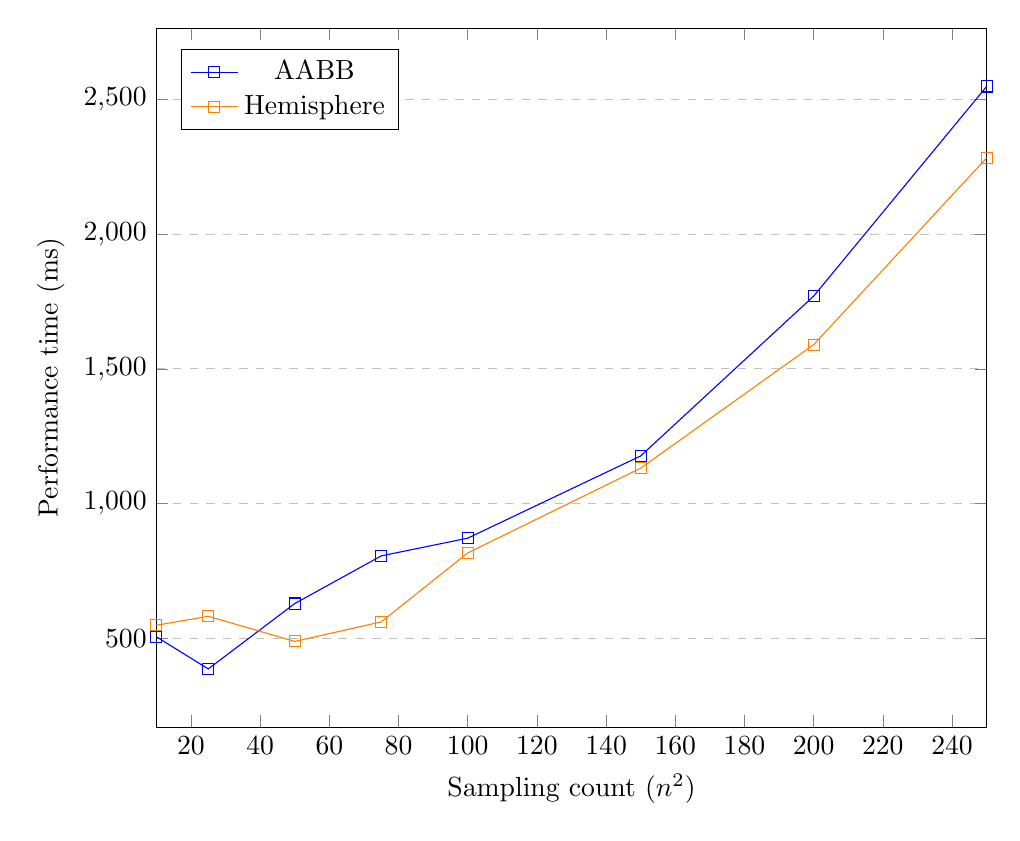
\begin{tikzpicture}
    \begin{axis}[
    width=\linewidth,
    xlabel={Sampling count ($n^2$)},
    ylabel={Performance time (ms)},
    xmin=10,
    xmax=250,
    legend pos=north west,
    ymajorgrids=true,
    grid style=dashed,
]
\addplot[color=blue, mark=square] coordinates {(10, 506.68)(25, 387.56)(50,629.92)(75,806.73)(100,872.39)(150,1177.29)(200,1769.80)(250,2547.22)};
\addplot[color=orange, mark=square] coordinates {(10, 549.48)(25, 582.76)(50,489.61)(75,561.96)(100,817.6)(150,1131.89)(200,1589.88)(250,2282.16)}; \legend{AABB,Hemisphere}
    \end{axis}
\end{tikzpicture}
        \caption{Performance time (ms)}
        \label{fig:graph_compare_sampling_method_performance_time}
    \end{subfigure}
    \hfill
    \begin{subfigure}[b]{0.9\linewidth}
        \centering
        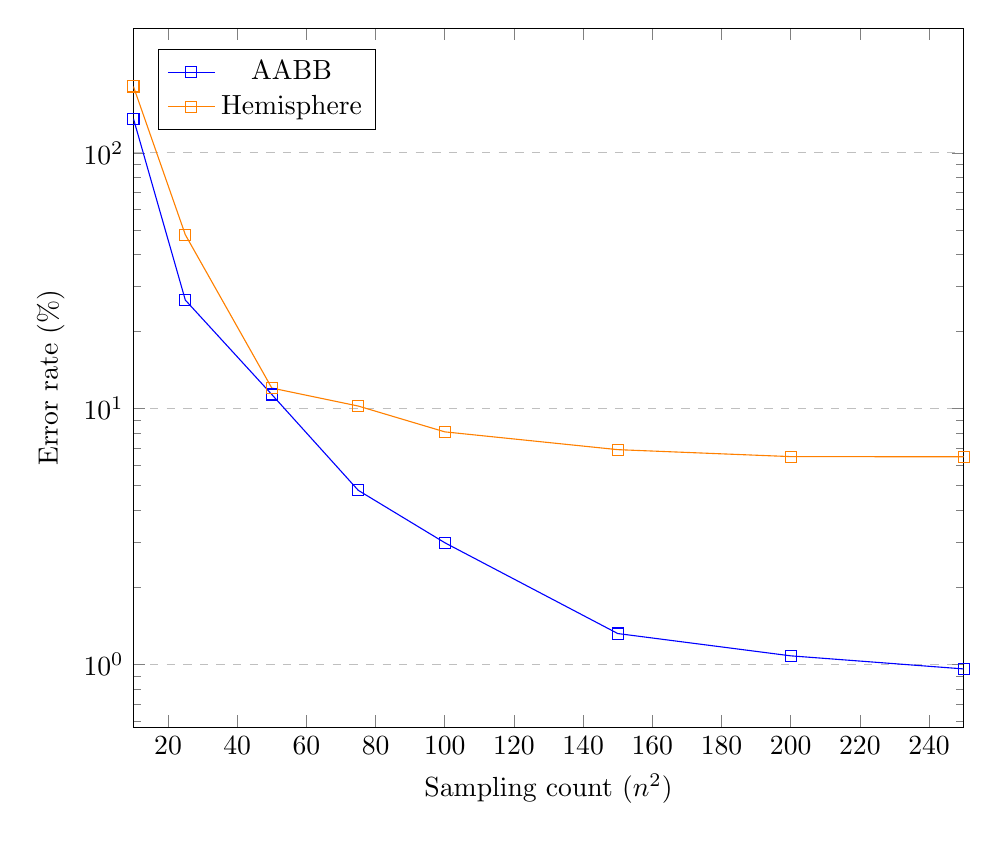
\begin{tikzpicture}
    \begin{axis}[
    width=\linewidth,
    xlabel={Sampling count ($n^2$)},
    ylabel={Error rate (\%)},
    xmin=10,
    xmax=250,
    legend pos=north west,
    ymajorgrids=true,
    grid style=dashed,
    ymode = log,
]
%\addplot[color=red, mark=square] coordinates {(10, 0.01)(25, 0.01)(50,0.01)(75,0.01)(100,0.01)(150,0.01)(200,0.01)(250,0.01)};
\addplot[color=blue, mark=square] coordinates {(10, 135.95)(25, 26.56)(50,11.35)(75,4.79)(100,2.99)(150,1.32)(200,1.08)(250,0.96)};
\addplot[color=orange, mark=square] coordinates {(10, 181.68)(25, 47.82)(50,12.03)(75,10.23)(100,8.11)(150,6.91)(200,6.49)(250,6.48)}; \legend{AABB,Hemisphere}
    \end{axis}
\end{tikzpicture}
        \caption{Error rate (\%)}\label{fig:graph_compare_sampling_method_error_rate}
    \end{subfigure}
    \caption{Compare the results of each sampling method according to the number of samples.
    }
    \label{fig:comparison_sampling_methods}
\end{figure}
}
%%%

It is important to note that processing time increases linearly with the number of samples (Fig.~\ref{fig:sampling_rate}).
Therefore, while the AABB sampling method can achieve similar accuracy at a sampling rate of 0.3\%, it requires much more processing time, negating the benefit of using RT-cores.
Furthermore, we found that the alternative sampling strategies increased the processing time of RT-HDIST by about 1.7 times compared to the vertex sampling method due to the added complexity of the sampling process.

%\DS{On considering}

\Skip{ %%%%%%%%%%%%%%%%%%%%%%%%%%%%%%%%%%%%%%%%%%%%%
\begin{table}[]
\caption{Comparison of the performance detailed between $baseline$ and $RTPD$. PSG means the penetration surface generation algorithms. Specifically, the PSG algorithms of $baseline$ assume the data existed on the GPU side. This result is computed on an average of 120 frames of Lucy benchmark in RTX 4080.}
\centering
\begin{tabular}{c|c|cc}
\hline
Step      & Detail             & $baseline$ & $RTPD$ \\
\hline
          & AS build           &  8132.32   &  516.14  \\
PIP       & Compute            &  10695.38   &  7.73  \\
          & Surface extraction &  76.65   &  20.85  \\
\hline
       & Data transfer (D $\to$ H)       &  0.81   & 0   \\
          & Vertex extraction  &  0   &  1.48  \\
PSG         & Compaction         & 0    &  4.11  \\
          & Mapping            &  61.60   & 0.49   \\
          & Data transfer (H $\to$ D)      & 0.72    & 0   \\
\hline
Hausdorff & AS build           &  342.71   & 2.96   \\
          & Compute            &  223.82   & 167.86  \\
\hline
\end{tabular}%
\label{table:step_analysis}
\end{table}

To verify our method's benefit in comparison to $baseline$ methods, we measured the processing times for each step of $baseline$ and $RTPD$. Table~\ref{table:step_analysis} shows the detailed performance time for Lucy benchmark in RTX 4080.

\paragraph{Penetration point extraction:}
We implemented the penetration point extraction step on CPU side and RT side, and we compared the algorithms. Table~\ref{table:step_analysis}-PIP shows the detailed results of each implementation. On the CPU side, the PIP algorithms's tree building process takes much time and trace time increases when the overlap region is bigger. However, on the RT side, tree building time (GAS build time) is accelerated by RT core. As a result, we get the time benefits for build time to \ToCheck{x15.76} times performance up. Another interesting fact is that the trace time of RT side required was only slightly increased compared to the increase in the overlap region. These results demonstrated a performance improvement of about \ToCheck{x1383.65} times over CPU about average trace time.

~\\

\paragraph{Penetration surface generation:}
To evaluate the performance of GPU-based penetration surface generation algorithms, we implement the CPU-based algorithms for this work. The CPU-based algorithms input the vertex index of penetration triangles to map structure simply and allocate the new vertex index. To compare the algorithms, we test two versions of the RTPD pipeline: the first one performs the RT-based PIP transfers the data to the CPU, and computes CPU-based penetration surface generation. On the contrary, the other one computes the GPU-based penetration surface generation algorithms without data transfer. 
Table~\ref{table:step_analysis}-PSG compares two versions of the penetration surface generation algorithms.
The proposed methods split the method into 3 steps (Vertex extraction, Compaction, and Mapping).
We also report each step's computational time of the GPU-based method.
As a result, the proposed methods achieve performance up \ToCheck{x10.40} times than CPU-based approaches.
Furthermore, the proposed GPU-based method has the advantage of minimizing communication with the CPU.

~\\
\paragraph{Hausdorff distance:} We also check the advantages of our approaches for Hausdorff distance.
Even though overall the number of vertices in the penetration surface is less than the number of ray samples, as seen in Table~\ref{table:step_analysis}-Hausdorff, our RT-based Hausdorff distance calculation methods are faster than Zheng's method~\cite{zheng2022economic}. In particular, when we compute the acceleration structure (AS) such as BVH, the RT-core gives benefits for the computational cost. In fact, we achieve the performance up \ToCheck{115.78} times for AS built time. This benefit becomes better as overlap ratio of the polygons increases. We only got \ToCheck{1.33} times for trace time and \ToCheck{3.31} times for total time performance up in this benchmark, but as the number of vertices in the penetration surface increases, the performance improvement is better. These results can be seen in section~\ref{section:overlap_test}.
~\\
} %%%%%%%%%%%%%%%%%%%%%%%%%%%%%%%%%%%%%%%%%%%%%%%%%%%%%%


\Skip{ %%%%%%%%%%%%%%%%%%%%%%%%%%%%%%%%%%%%%%%%%
\subsection{Overlap region test}
\label{section:overlap_test}

\begin{figure}[h]
    \centering
    \begin{subfigure}[b]{0.9\linewidth}
        \centering
    \begin{tikzpicture}
    \begin{axis}[
    width=\linewidth,
    %xtick=data,
    %xticklabels from table={Context/Rawdata/overlap_ratio_performance.csv}{ratio},
    xlabel={Overlap ratio (\%)},
    ylabel={Execution time (ms)},
    %xmin=0,
    %xmax=50,
    legend pos=north east,
    ymajorgrids=true,
    grid style=dashed,
    ymode=log,
]
%\addplot table [x=Step, y=A, col sep=comma] {Context/Rawdata/simple_test.csv};
\addplot[color=blue,  mark=square] table [x=Rate, y=sh_cpu, col sep=comma] {Context/Rawdata/overlapPerf.csv};
\addplot[color=brown, mark=square] table [x=Rate, y=sh_nv, col sep=comma] {Context/Rawdata/overlapPerf.csv};
\addplot[color=orange,mark=square] table [x=Rate, y=sh_rt, col sep=comma] {Context/Rawdata/overlapPerf.csv};
%\addplot+ table [x=ratio, y=blnv, col sep=comma] {Context/Rawdata/overlap_ratio_performance.csv};
%\addplot+ table [x=ratio, y=blrt, col sep=comma] {Context/Rawdata/overlap_ratio_performance.csv}; 
\legend{$baseline$,$GPU_{naive}$,$RTPD$}
    \end{axis}
\end{tikzpicture}
\caption{Total}
\end{subfigure}
\begin{subfigure}[b]{0.9\linewidth}
        \centering
    \begin{tikzpicture}
    \begin{axis}[
    width=\linewidth,
    %xtick=data,
    %xticklabels from table={Context/Rawdata/overlap_ratio_performance.csv}{ratio},
    xlabel={Overlap ratio (\%)},
    ylabel={Execution time (ms)},
    %xmin=0,
    %xmax=50,
    legend pos=north east,
    ymajorgrids=true,
    grid style=dashed,
    ymode=log,
]
%\addplot table [x=Step, y=A, col sep=comma] {Context/Rawdata/simple_test.csv};
\addplot[color=blue,  mark=square] table [x=Rate, y=sh_cpu, col sep=comma] {Context/Rawdata/overlapPerf_PIP.csv};
%\addplot[color=brown, mark=square] table [x=Rate, y=sh_nv, col sep=comma] {Context/Rawdata/overlapPerf_PIP.csv};
\addplot[color=orange,mark=square] table [x=Rate, y=sh_rt, col sep=comma] {Context/Rawdata/overlapPerf_PIP.csv};
%\addplot+ table [x=ratio, y=blnv, col sep=comma] {Context/Rawdata/overlap_ratio_performance.csv};
%\addplot+ table [x=ratio, y=blrt, col sep=comma] {Context/Rawdata/overlap_ratio_performance.csv}; 
\legend{$baseline$,$RTPD$}
    \end{axis}
\end{tikzpicture}
\caption{PIP}
\end{subfigure}
\begin{subfigure}[b]{0.9\linewidth}
        \centering
    \begin{tikzpicture}
    \begin{axis}[
    width=\linewidth,
    %xtick=data,
    %xticklabels from table={Context/Rawdata/overlap_ratio_performance.csv}{ratio},
    xlabel={Overlap ratio (\%)},
    ylabel={Execution time (ms)},
    %xmin=0,
    %xmax=50,
    legend pos=north east,
    ymajorgrids=true,
    grid style=dashed,
    ymode=log,
]
%\addplot table [x=Step, y=A, col sep=comma] {Context/Rawdata/simple_test.csv};
\addplot[color=blue,  mark=square] table [x=Rate, y=sh_cpu, col sep=comma] {Context/Rawdata/overlapPerf_Hdist.csv};
\addplot[color=brown, mark=square] table [x=Rate, y=sh_nv, col sep=comma] {Context/Rawdata/overlapPerf_Hdist.csv};
\addplot[color=orange,mark=square] table [x=Rate, y=sh_rt, col sep=comma] {Context/Rawdata/overlapPerf_Hdist.csv};
%\addplot+ table [x=ratio, y=blnv, col sep=comma] {Context/Rawdata/overlap_ratio_performance.csv};
%\addplot+ table [x=ratio, y=blrt, col sep=comma] {Context/Rawdata/overlap_ratio_performance.csv}; 
\legend{$baseline$,$GPU_{naive}$,$RTPD$}
    \end{axis}
\end{tikzpicture}
\caption{Hausdorff}
\end{subfigure}
    \caption{The execution time of penetration depth as changes overlap ratio of $stmatthew_{High}$. $GPU_{naive}$ is brute force Hausdorff computation on GPU. We use the $PIP_{RT}$ for this test.}
    \label{fig:overlap_performance}
\end{figure}

To confirm the tendency of changes in overlap regions, we implemented and tested the special benchmark on RTX 4080. We computed the transformation to the X-axis so that the overlap region was 10, 20, 30, 40, and 50\% per each polygon.
The figure~\ref{fig:overlap_performance} presents the graph of changes in execution time according to the overlap ratio for $stmatthew_{High}$.
We found that the executive time increases as the overlap ratio. While the PIP performance is almost maintained, the Hausdorff distance is changed greatly because the Hausdorff distance is dependent on the penetration surface.
As a result, we confirm the performance of Hausdorff distance \ToCheck{4.97} times to \ToCheck{5.68} times slightly up as the overlap ratio increased than $baseline$.
This tendency demonstrates that our method is more efficient as the overlap ratio increases for the huge model.

\TODO{Time graph has too much gap. How does change to the "amount of change" graph?}


\subsection{Comparison of sampling methods}

To evaluate the impact of AABB sampling methods, we implemented both sampling methods $RTHD_{Hemisphere}$ and $RTHD_{AABB}$ and brute force Hausdorff distance method $HD_{GPU_{Naive}}$ on the GPU. Also, we set the benchmark $Lucy$ with sampling counts 10, 25, 50, 75, 100, 150, 200, and 250. 
%We evaluate the sampling method's accuracy and performance in comparison to $HD_{GPU_{Naive}}$.
Figure~\ref{fig:comparison_sampling_methods} presents the change of results when the sample increased.

\begin{figure}[t]
    \centering
    \includegraphics[width=0.8\columnwidth]{Image/graphs/sampling_method.pdf}
    \caption{These graphs display changes in error rates as the sampling rate increases for three different sampling strategies in the $Lucy$ benchmark with a 0.5 overlap ratio.}
    \label{fig_sampling_method}
\end{figure}
%
%
\Skip{
\begin{figure}[t]
    \centering
    \begin{subfigure}[b]{0.9\linewidth}
        \centering
       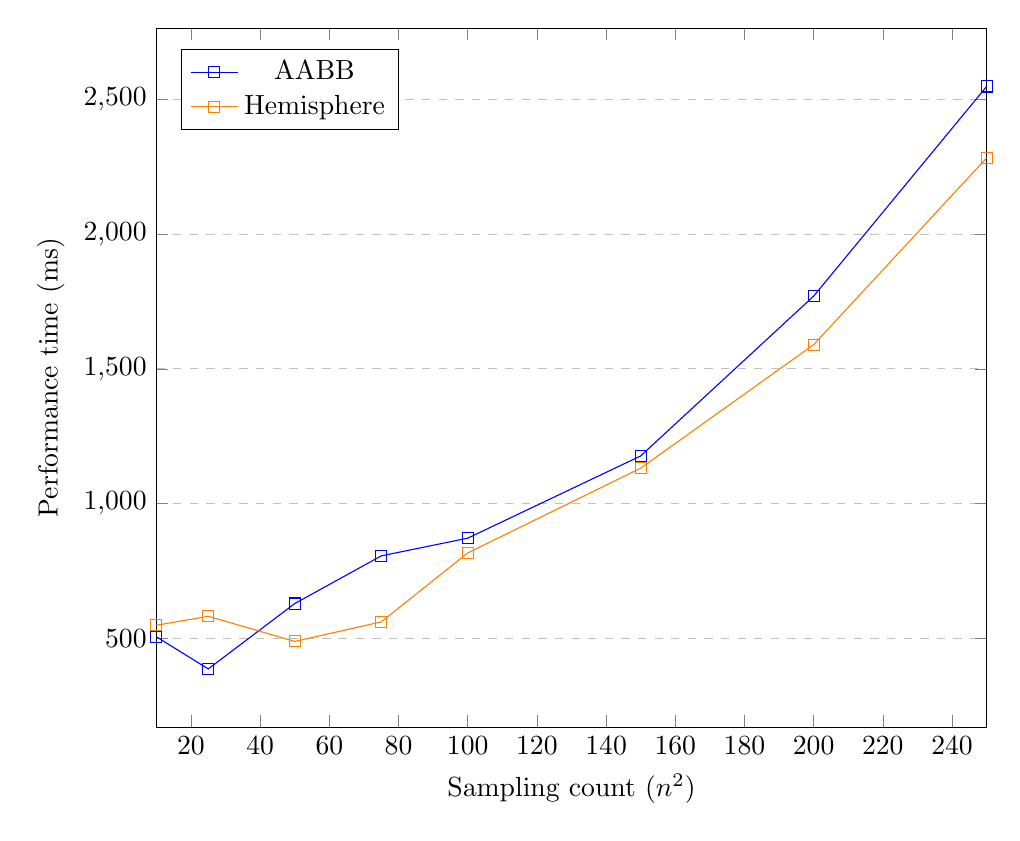
\begin{tikzpicture}
    \begin{axis}[
    width=\linewidth,
    xlabel={Sampling count ($n^2$)},
    ylabel={Performance time (ms)},
    xmin=10,
    xmax=250,
    legend pos=north west,
    ymajorgrids=true,
    grid style=dashed,
]
\addplot[color=blue, mark=square] coordinates {(10, 506.68)(25, 387.56)(50,629.92)(75,806.73)(100,872.39)(150,1177.29)(200,1769.80)(250,2547.22)};
\addplot[color=orange, mark=square] coordinates {(10, 549.48)(25, 582.76)(50,489.61)(75,561.96)(100,817.6)(150,1131.89)(200,1589.88)(250,2282.16)}; \legend{AABB,Hemisphere}
    \end{axis}
\end{tikzpicture}
        \caption{Performance time (ms)}
        \label{fig:graph_compare_sampling_method_performance_time}
    \end{subfigure}
    \hfill
    \begin{subfigure}[b]{0.9\linewidth}
        \centering
        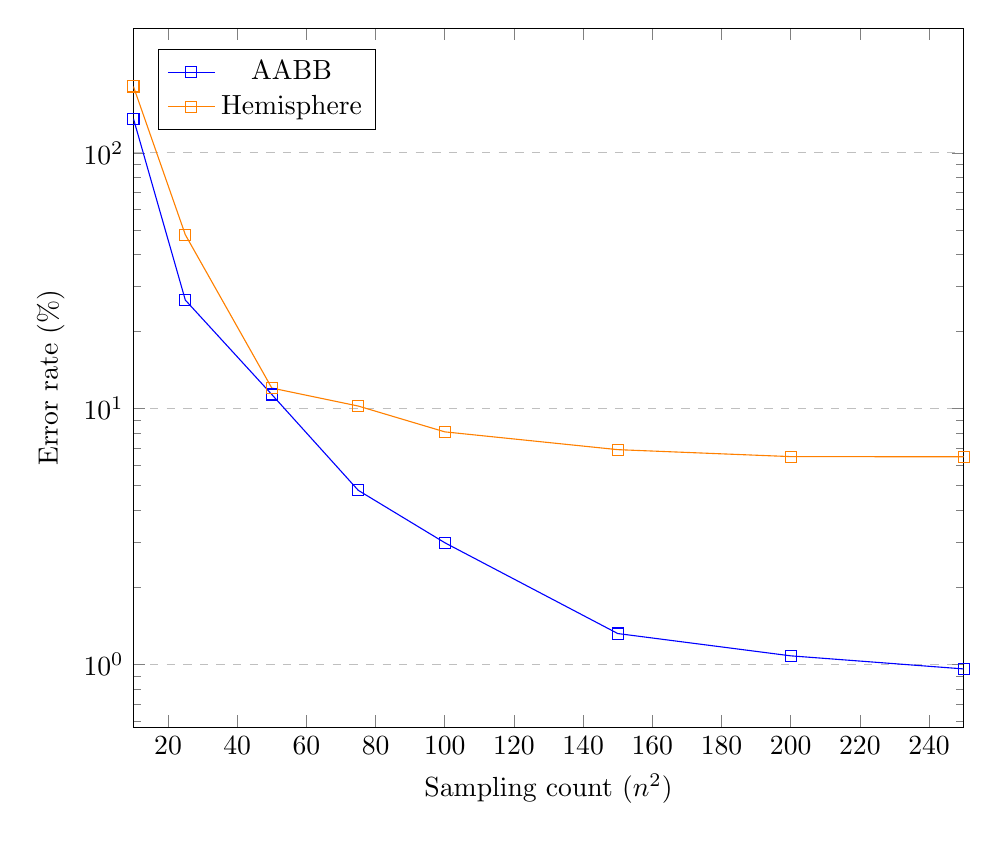
\begin{tikzpicture}
    \begin{axis}[
    width=\linewidth,
    xlabel={Sampling count ($n^2$)},
    ylabel={Error rate (\%)},
    xmin=10,
    xmax=250,
    legend pos=north west,
    ymajorgrids=true,
    grid style=dashed,
    ymode = log,
]
%\addplot[color=red, mark=square] coordinates {(10, 0.01)(25, 0.01)(50,0.01)(75,0.01)(100,0.01)(150,0.01)(200,0.01)(250,0.01)};
\addplot[color=blue, mark=square] coordinates {(10, 135.95)(25, 26.56)(50,11.35)(75,4.79)(100,2.99)(150,1.32)(200,1.08)(250,0.96)};
\addplot[color=orange, mark=square] coordinates {(10, 181.68)(25, 47.82)(50,12.03)(75,10.23)(100,8.11)(150,6.91)(200,6.49)(250,6.48)}; \legend{AABB,Hemisphere}
    \end{axis}
\end{tikzpicture}
        \caption{Error rate (\%)}\label{fig:graph_compare_sampling_method_error_rate}
    \end{subfigure}
    \caption{Compare the results of each sampling method according to the number of samples.
    }
    \label{fig:comparison_sampling_methods}
\end{figure}
}

The ray sampling time takes very little time (<=0.1\% of the total processing time) regardless of sampling count, but the total computation time linearly increases as shown in the graph. Besides the error rate decreases as the sample increases. In this benchmark, we found that the result converges in about 10,000 ray samples. In fact, $RTHD_{AABB}$ has an error rate of less than 3\% in 10000 samples. On the other hand, $RTHD_{Hemisphere}$ also converges but the error rate does not decrease more than \ToCheck{6.4}\%. This means the ray of $RTHD_{Hemisphere}$ has not been sampled in a valid direction. As a result, $RTHD_{AABB}$ achieves more accurate results within the same time at the same number of samples than $RTHD_{Hemisphere}$. This result demonstrates the efficiency of our method $RTHD_{AABB}$.
} %%%%%%%%%%%%%%%%%%%%%%%%%%%%%%%%%%%%%%%%%

%\Skip{ %%%%%%%%%%%%%%%%%%%%%%%%%%%%%%%%%%%%%%%%%
\subsection{Ablation study} 

To evaluate the contribution of each component of our method to overall performance improvement, we conducted an ablation study using the $Lucy$ benchmark on an RTX 3080.
The results are shown in Table~\ref{table_ablation}.
For \revision{PPE} and HDIST, the baselines are CUDA-based implementations from $GPU_{cuda}$.
For PSG, the baseline is the CPU implementation, as we propose a GPU-based PSG algorithm in this work (Sec.~\ref{subsec:surfaceGen}).
%%%
\begin{table}[t!]
\centering
\scriptsize
\caption{The ablation study results of \name using LLaMA3-8B-Instruct as the base model on the TFV task. \textcolor{Maroon}{Red} signifies degradation in percentage.}
\resizebox{\columnwidth}{!}{
\begin{tabular}{lllll}
\toprule
 \multirow{2}{*}[-0.5ex]{\textbf{Methods}} & \multicolumn{4}{c}{\textbf{\;\;TFV}} \\
\cmidrule(l){2-5}
 &\bf\%Acc. &\bf\%F1 &\bf\%Prec. &\bf\%Recall \\
\midrule
 \rowcolor{myblue} \textbf{\name (Ours)} &77.20  \basex{0.00} &77.46 \basex{0.00} &79.98 \basex{0.00} &77.20  \basex{0.00}  \\ 
  % w/o LoRA &- \downbad{0.0} &- \downbad{0.0} &- \downbad{0.0} &- \downbad{0.0} \\
  w/o PHL &70.96 \downbad{6.24} &70.86 \downbad{6.60} &71.35 \downbad{8.63} &70.96 \downbad{6.24}\\
  w/o PHL, w/ HGNN &72.70 \downbad{4.50} &72.54 \downbad{4.92} &73.03 \downbad{6.95} &72.70 \downbad{4.50}\\
  w/o Inquiry Emb. & 72.63 \downbad{4.57} & 73.39 \downbad{4.07} & 74.22 \downbad{5.76} & 74.22 \downbad{2.98}\\

\bottomrule
\end{tabular}}
\label{tab:ablation_study}
\vspace{-0.1in}
\end{table}

%%%

As shown in rows 2 to 4 of Table~\ref{table_ablation}, all components contribute to reducing the total processing time.
Among the three, the RT-based HDIST algorithm has the greatest impact, reducing processing time by about 26\% on average.
The GPU-based PSG algorithm also plays a critical role, achieving the highest relative performance improvement compared to the baseline, despite having the smallest workload (Table~\ref{table:breakdown}), with an average reduction of 24\%.
While the RT-based PPE contributes the least to overall performance, it still consistently reduces total processing time by about 8\% on average across all tested cases.

As we incorporate more components from our method, the performance improves significantly compared to using just one component. Specifically, types 5, 6, and 7 reduce the total processing time by approximately 33\%, 51\%, and 50\% on average, respectively.
Finally, the full version of our method (type 8, $RTPD$) achieves the best performance, reducing the processing time by about 69\% on average.

Although $RTPD$ is an approximate penetration depth algorithm due to its sample-based HDIST computation, our method can be applied only to the PPE and PSG stages while using the CUDA-based HDIST method if an application requires exact results.
This approach is demonstrated in type 5 of Table~\ref{table_ablation}, which still improves performance by 1.50 times on average over the baseline (type 1).
These results demonstrate that the components of our method can be selectively applied to various applications based on specific requirements, leading to improved performance.

\Skip{ %%%%%%%%%%%%%%%%%%%%%%%%%%%%%%%%%%%%%%%%%
Table~\ref{table:Ablation study} presents the result of implementation that applies our methods for each step.
Specifically, our RT-based PIP methods have a lot more benefits than $baseline$'s PIP (almost \ToCheck{x10.28} times faster. It can compute compared with test type 6 and RTPD).
In a similar manner, we can compute the benefit of the penetration surface generation method and RT-based Hausdorff distance, they achieve \ToCheck{x2.24} and \ToCheck{x8.91} times faster.
On the other hand, the accuracy (error rate) of $baseline$ is better than our methods (See $baseline$ and test types 1,2,4).
Instead, we save the execution times at the expense of accuracy (We get times up \ToCheck{x18.57} times than $baseline$ and lose the accuracy by \ToCheck{1.49}\%). 
These results demonstrate that our RT-based method is more efficient than $baseline$ methods.
} %%%%%%%%%%%%%%%%%%%%%%%%%%%%%%%%%%%%%%%%%


%On lucy dataset--> x25.72/x32.26/x45.81/x57.27
%RT cores --> 0/46/68/76
%\subsubsection{Scalability}

